\documentclass{beamer}
\mode<presentation>
\usepackage{amsmath}
\usepackage{amssymb}
%\usepackage{advdate}
\usepackage{adjustbox}
\usepackage{subcaption}
\usepackage{enumitem}
\usepackage{multicol}
\usepackage{mathtools}
\usepackage{listings}
\usepackage{float}
\usepackage{graphicx}
\usepackage{url}
\def\UrlBreaks{\do\/\do-}
\usetheme{Boadilla}
\usecolortheme{lily}
\setbeamertemplate{footline}
{
  \leavevmode%
  \hbox{%
  \begin{beamercolorbox}[wd=\paperwidth,ht=2.25ex,dp=1ex,right]{author in head/foot}%
    \insertframenumber{} / \inserttotalframenumber\hspace*{2ex} 
  \end{beamercolorbox}}%
  \vskip0pt%
}
\setbeamertemplate{navigation symbols}{}

\providecommand{\nCr}[2]{\,^{#1}C_{#2}} % nCr
\providecommand{\nPr}[2]{\,^{#1}P_{#2}} % nPr
\providecommand{\mbf}{\mathbf}
\providecommand{\pr}[1]{\ensuremath{\Pr\left(#1\right)}}
\providecommand{\qfunc}[1]{\ensuremath{Q\left(#1\right)}}
\providecommand{\sbrak}[1]{\ensuremath{{}\left[#1\right]}}
\providecommand{\lsbrak}[1]{\ensuremath{{}\left[#1\right.}}
\providecommand{\rsbrak}[1]{\ensuremath{{}\left.#1\right]}}
\providecommand{\brak}[1]{\ensuremath{\left(#1\right)}}
\providecommand{\lbrak}[1]{\ensuremath{\left(#1\right.}}
\providecommand{\rbrak}[1]{\ensuremath{\left.#1\right)}}
\providecommand{\cbrak}[1]{\ensuremath{\left\{#1\right\}}}
\providecommand{\lcbrak}[1]{\ensuremath{\left\{#1\right.}}
\providecommand{\rcbrak}[1]{\ensuremath{\left.#1\right\}}}
\theoremstyle{remark}
\newtheorem{rem}{Remark}
\newcommand{\sgn}{\mathop{\mathrm{sgn}}}
\providecommand{\abs}[1]{\left\vert#1\right\vert}
\providecommand{\res}[1]{\Res\displaylimits_{#1}} 
\providecommand{\norm}[1]{\lVert#1\rVert}
\providecommand{\mtx}[1]{\mathbf{#1}}
\providecommand{\mean}[1]{E\left[ #1 \right]}
\providecommand{\fourier}{\overset{\mathcal{F}}{ \rightleftharpoons}}
%\providecommand{\hilbert}{\overset{\mathcal{H}}{ \rightleftharpoons}}
\providecommand{\system}{\overset{\mathcal{H}}{ \longleftrightarrow}}
	%\newcommand{\solution}[2]{\textbf{Solution:}{#1}}
%\newcommand{\solution}{\noindent \textbf{Solution: }}
\providecommand{\dec}[2]{\ensuremath{\overset{#1}{\underset{#2}{\gtrless}}}}
\newcommand{\myvec}[1]{\ensuremath{\begin{pmatrix}#1\end{pmatrix}}}
\let\vec\mathbf

\lstset{
language=C,
frame=single, 
breaklines=true,
columns=fullflexible
}

\numberwithin{equation}{section}

\title{Presentation - Matgeo}
\author{Aryansingh Sonaye \\
AI25BTECH11032 \\
EE1030 - Matrix Theory}

\date{\today} 
\begin{document}

\begin{frame}
\titlepage
\end{frame}

\section{Problem}
\begin{frame}
\frametitle{Problem Statement}
\textbf{Problem 9.8.34}
Find the equation of the line passing through the points of intersection of the circles
\begin{align}
3x^2+3y^2-2x+12y-9=0
\quad\text{and}\quad
x^2+y^2+6x+2y-15=0.
\end{align}


\end{frame}

\section{Solution}
\subsection{Description of Variables used}
\begin{frame}
\frametitle{Description of Variables used}
The general conic is
\begin{align}
\vec{x}^\top V \vec{x} + 2\vec{u}^\top \vec{x} + f = 0, 
\quad \vec{x}=\myvec{x\\y}.
\end{align}

\begin{table}[H]
\centering
\begin{tabular}{|c|c|c|}
\hline
 & $C_1$ & $C_2$ \\
\hline
$V$ & $\myvec{3 & 0 \\ 0 & 3}$ & $\myvec{1 & 0 \\ 0 & 1}$ \\
\hline
$\vec{u}$ & $\myvec{-1 \\ 6}$ & $\myvec{3 \\ 1}$ \\
\hline
$f$ & $-9$ & $-15$ \\
\hline
\end{tabular}
\end{table}


\end{frame}

\subsection{Theoretical Solution }
\begin{frame}
\frametitle{Theoretical Solution}
All conics through the intersection points are given by the locus
\begin{align}
\vec{x}^\top (V_1+\mu V_2)\vec{x}
+2(\vec{u}_1+\mu\vec{u}_2)^\top\vec{x}
+(f_1+\mu f_2) &= 0.
\end{align}

Since we want a line, we eliminate the quadratic part by choosing $\mu$ such that
\begin{align}
V_1+\mu V_2 &= (3+\mu)I = 0, \\
\mu &= -3.
\end{align}

Substituting $\mu=-3$, the equation of the required line becomes
\begin{align}
2(\vec{u}_1-3\vec{u}_2)^\top \vec{x} + (f_1-3f_2) &= 0.
\end{align}

\end{frame}

\begin{frame}
\frametitle{Theoretical Solution}
Now we compute the coefficients:
\begin{align}
\vec{u}_1-3\vec{u}_2 &= \myvec{-1\\6} - 3\myvec{3\\1} = \myvec{-10\\3}, \\
f_1-3f_2 &= -9 - 3(-15) = 36.
\end{align}

Thus the line is
\begin{align}
2\myvec{-10 & 3}\vec{x} + 36 &= 0.
\end{align}

Multiplying throughout by $-\tfrac{1}{2}$, we obtain
\begin{align}
\myvec{10\\-3}^\top \vec{x} - 18 &= 0.
\end{align}

\begin{align}
\boxed{\myvec{10\\-3}^\top \vec{x} - 18 = 0}
\end{align}

This is the required line through the intersection points.


\end{frame}


\subsection{Plot}
\begin{frame}
    \frametitle{Plot}
\begin{figure}[H]
   \centering
   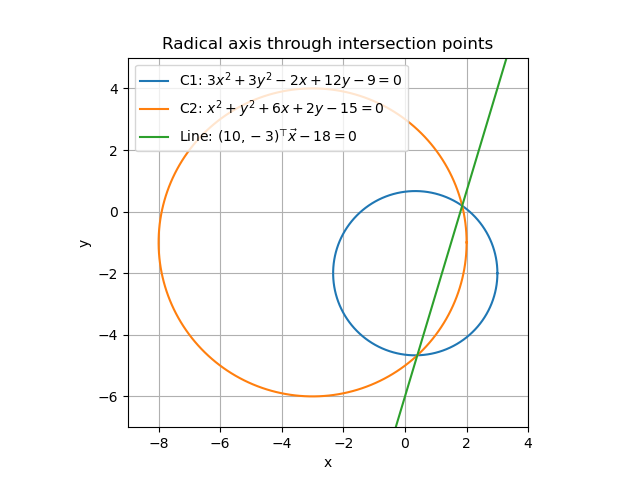
\includegraphics[width=0.8\columnwidth]{figs/radical.png}
   \caption{}
   \label{}
   \end{figure}
\end{frame}

\begin{frame}[fragile]
    \frametitle{Code - C}
    \begin{lstlisting}
// Compute radical axis of two circles in conic form
// Circle: x^T V x + 2u^T x + f = 0 with V = a I
// Input: a1,u1,f1 and a2,u2,f2
// Output: line L^T x + c = 0 (L is size 2, c scalar)

void radical_axis(
    double a1, const double u1[2], double f1,
    double a2, const double u2[2], double f2,
    double L_out[2], double *c_out
) {
    double mu = -a1 / a2; // value that cancels quadratic part
    L_out[0] = 2.0 * (u1[0] + mu * u2[0]);
    L_out[1] = 2.0 * (u1[1] + mu * u2[1]);
    *c_out    =       (f1     + mu * f2);
}


    \end{lstlisting}
    \end{frame}


\begin{frame}[fragile]
    \frametitle{Code - Python(with shared C code)}
    The code to obtain the required plot is
    \begin{lstlisting}
import ctypes as ct
import numpy as np
import matplotlib.pyplot as plt

# 1) load the shared library (same folder)
lib = ct.CDLL("./libradical_simple.so")

# 2) tell ctypes the C signature
# void radical_axis(double a1, const double u1[2], double f1,
#                   double a2, const double u2[2], double f2,
#                   double L_out[2], double *c_out);
lib.radical_axis.argtypes = [
    ct.c_double,                          # a1
    ct.POINTER(ct.c_double), ct.c_double, # u1, f1
    ct.c_double,                          # a2
    ct.POINTER(ct.c_double), ct.c_double, # u2, f2

\end{lstlisting}
\end{frame}
\begin{frame}[fragile]
\frametitle{Code - Python(with shared C code)}
\begin{lstlisting}
    ct.POINTER(ct.c_double),              # L_out
    ct.POINTER(ct.c_double)               # c_out
]
lib.radical_axis.restype = None

# 3) problem data (Problem 9.8.34)
a1 = 3.0
u1 = np.array([-1.0, 6.0], dtype=np.double)
f1 = -9.0
a2 = 1.0
u2 = np.array([3.0, 1.0], dtype=np.double)
f2 = -15.0

# 4) outputs
L = np.zeros(2, dtype=np.double)
c = ct.c_double()   # <-- IMPORTANT: ctypes double, so we can pass byref



\end{lstlisting}
\end{frame}

\begin{frame}[fragile]
\frametitle{Code - Python(with shared C code)}
\begin{lstlisting}
# 5) call C
lib.radical_axis(
    a1, u1.ctypes.data_as(ct.POINTER(ct.c_double)), f1,
    a2, u2.ctypes.data_as(ct.POINTER(ct.c_double)), f2,
    L.ctypes.data_as(ct.POINTER(ct.c_double)),
    ct.byref(c)  # pass the address of the ctypes double
)

print("Raw line from C: L =", L, "  c =", c.value)

# 6) scale to nice integers: (10, -3)^T x - 18 = 0
scale = -0.5  # because C gives L=[-20,6], c=36
L_scaled = L * scale
c_scaled = c.value * scale
print(f"Vector form: ({int(L_scaled[0])} \\\\ {int(L_scaled[1])})^T x {c_scaled:+.0f} = 0")



\end{lstlisting}
\end{frame}

\begin{frame}[fragile]
\frametitle{Code - Python(with shared C code)}
\begin{lstlisting}
# 7) plot circles + line
def circle_center_radius(a, u, f):
    # V = a I; center = -u/a; r^2 = ||u||^2/a^2 - f/a
    center = -u / a
    r2 = (u @ u) / (a*a) - f / a
    return center, np.sqrt(r2)

c1, r1 = circle_center_radius(a1, u1, f1)
c2, r2 = circle_center_radius(a2, u2, f2)
theta = np.linspace(0, 2*np.pi, 400)
x1 = c1[0] + r1*np.cos(theta); y1 = c1[1] + r1*np.sin(theta)
x2 = c2[0] + r2*np.cos(theta); y2 = c2[1] + r2*np.sin(theta)

xmin = min(c1[0]-r1, c2[0]-r2) - 1
xmax = max(c1[0]+r1, c2[0]+r2) + 1
ymin = min(c1[1]-r1, c2[1]-r2) - 1
ymax = max(c1[1]+r1, c2[1]+r2) + 1

\end{lstlisting}
\end{frame}

\begin{frame}[fragile]
\frametitle{Code - Python(with shared C code)}
\begin{lstlisting}
xx = np.linspace(xmin, xmax, 600)
if abs(L_scaled[1]) > 1e-12:
    yy = (-c_scaled - L_scaled[0]*xx) / L_scaled[1]
else:
    xx = np.full_like(xx, -c_scaled / L_scaled[0])
    yy = np.linspace(ymin, ymax, 600)
plt.figure()
plt.plot(x1, y1, label="C1: $3x^2+3y^2-2x+12y-9=0$")
plt.plot(x2, y2, label="C2: $x^2+y^2+6x+2y-15=0$")
plt.plot(xx, yy, label=r"Line: $(10,-3)^\top \vec{x} - 18 = 0$")
plt.gca().set_aspect('equal', adjustable='box')
plt.xlim(xmin, xmax); plt.ylim(ymin, ymax)
plt.grid(True); plt.legend()
plt.title("Radical axis through intersection points")
plt.xlabel("x"); plt.ylabel("y")
plt.savefig("radical.png")
plt.show()

\end{lstlisting}
\end{frame}



\begin{frame}[fragile]
\frametitle{Code - Python only}
\begin{lstlisting}
import numpy as np
import matplotlib.pyplot as plt

# Circles:
# C1: 3x^2 + 3y^2 - 2x + 12y - 9 = 0
a1 = 3.0
u1 = np.array([-1.0, 6.0])
f1 = -9.0
# C2: x^2 + y^2 + 6x + 2y - 15 = 0
a2 = 1.0
u2 = np.array([3.0, 1.0])
f2 = -15.0

# ---- Find radical axis (line through intersections) ----
mu = -a1/a2
L = 2*(u1 + mu*u2)   # vector
c = f1 + mu*f2       # scalar




\end{lstlisting}
\end{frame}

\begin{frame}[fragile]
\frametitle{Code - Python only}
\begin{lstlisting}
print("Line (raw):", L, ". x +", c, "= 0")

# Scale to nice integers
L = -0.5*L
c = -0.5*c
print("Final line:", f"({int(L[0])} \\\\ {int(L[1])})^T x {int(c):+d} = 0")

# ---- Plot circles and line ----
theta = np.linspace(0, 2*np.pi, 400)

# Circle 1
center1 = -u1/a1
r1 = np.sqrt((u1@u1)/(a1*a1) - f1/a1)
x1 = center1[0] + r1*np.cos(theta)
y1 = center1[1] + r1*np.sin(theta)


\end{lstlisting}
\end{frame}

\begin{frame}[fragile]
\frametitle{Code - Python only}
\begin{lstlisting}
# Circle 2
center2 = -u2/a2
r2 = np.sqrt((u2@u2)/(a2*a2) - f2/a2)
x2 = center2[0] + r2*np.cos(theta)
y2 = center2[1] + r2*np.sin(theta)
# Line points
xx = np.linspace(min(center1[0]-r1, center2[0]-r2)-1,
                 max(center1[0]+r1, center2[0]+r2)+1, 600)
yy = (-c - L[0]*xx)/L[1]

plt.plot(x1, y1, label="C1")
plt.plot(x2, y2, label="C2")
plt.plot(xx, yy, label="Radical axis")
plt.gca().set_aspect('equal', adjustable='box')
plt.legend(); plt.grid(True)
plt.savefig("newradical.png")
plt.show()




\end{lstlisting}
\end{frame}

\end{document}
